\documentclass[12pt]{article}
\usepackage[utf8]{inputenc}
\usepackage[T1]{fontenc}
\usepackage[a4paper, margin=1in]{geometry}
\usepackage{xcolor}
\usepackage{titlesec}
\usepackage{lmodern}
\usepackage{amsmath, amssymb}
\usepackage{enumitem}
\usepackage{graphicx}
\usepackage{pdfpages}
\usepackage{fancyhdr}
\usepackage{float}
\usepackage{hyperref}


\definecolor{chaptercolor}{RGB}{0, 51, 102} 
\definecolor{sectioncolor}{RGB}{0, 102, 102}   
\definecolor{subsectioncolor}{RGB}{60, 60, 60}  


\titleformat{\section}
  {\normalfont\Large\bfseries\color{chaptercolor}}{\thesection}{1em}{}
\titlespacing*{\section}{0pt}{20pt}{10pt}
\titleformat{\subsection}
  {\normalfont\large\bfseries\color{sectioncolor}}{\thesubsection}{1em}{}
\titlespacing*{\subsection}{0pt}{15pt}{8pt}
\titleformat{\subsubsection}
  {\normalfont\normalsize\bfseries\color{subsectioncolor}}{\thesubsubsection}{1em}{}
\titlespacing*{\subsubsection}{0pt}{12pt}{6pt}


\title{\textbf{Dynamical Mass Estimation of a Galaxy Cluster at Redshift 0.08}}
\author{Pranauv C.H}
\date{}


\setlength{\headheight}{15pt} 
\pagestyle{fancy}
\fancyhf{}
\fancyhead[R]{Dynamical Mass Estimation of a Galaxy Cluster}
\fancyfoot[C]{\thepage}

\begin{document}

\maketitle

\begin{abstract}
Galaxy clusters are among the largest gravitationally bound systems in the Universe, and their masses provide crucial insights into l
arge-scale structure formation and dark matter content. In this work, we estimate the dynamical mass of a galaxy cluster using 
spectroscopic data from the Sloan Digital Sky Survey (SDSS). After applying a $3\sigma$ clipping method to filter non-member galaxies, 
a final sample of 91 galaxies was obtained. The cluster redshift was determined to be $z \approx 0.0801$ with a velocity dispersion 
of $1316 \pm 99$ km s$^{-1}$. Using the virial theorem, the dynamical mass was calculated as $(6.9 \pm 1.4) \times 10^{14} M_\odot$, 
consistent with expectations for rich clusters. This analysis highlights the effectiveness of redshift-based membership selection and 
velocity dispersion measurements in probing the gravitational potential of galaxy clusters, and demonstrates the utility of SDSS data 
for cluster dynamics studies.
\end{abstract}

\newpage
\tableofcontents

\newpage
\section{Introduction}

Galaxy clusters are the most massive gravitationally bound structures in the universe, comprising hundreds to thousands of galaxies, 
hot gas, and dark matter. Understanding their mass distribution is crucial for probing the nature of dark matter and the large-scale 
structure of the cosmos. The dynamical mass estimation of galaxy clusters, particularly at moderate redshifts, provides valuable insights 
into their formation and evolution.\\
\\
In this study, we focus on a galaxy cluster at redshift $z \approx 0.08$, selected through a 3$\sigma$ filtering of redshift measurements. 
The velocity dispersion of the cluster, approximately 1316 km/s, indicates a massive system in a state of gravitational equilibrium. 
By applying the virial theorem, we estimate the cluster's dynamical mass to be $6.89 \times 10^{14} M_\odot$, consistent with the mass 
range of rich clusters observed in the local universe.\\
\\
The application of the virial theorem to clusters of galaxies was first introduced by Zwicky (1937), who utilized the observed velocities 
of galaxies within the Coma cluster to estimate its mass, leading to the recognition of the significant presence of dark matter in such systems. 
This foundational work has paved the way for subsequent studies employing various methods, including X-ray observations and gravitational lensing, 
to estimate cluster masses.\\
\\
The analysis presented herein utilizes Python-based tools such as Astropy, pandas, Matplotlib, and SciPy for data handling, statistical analysis, and visualization. 
These tools facilitate the processing of redshift and positional data, the computation of velocity dispersions, and the estimation of dynamical masses, ensuring a 
robust and reproducible methodology.\\
\\
This report aims to provide a comprehensive dynamical mass estimate of a galaxy cluster at moderate redshift, contributing to the broader understanding of cluster 
properties and the role of dark matter in their formation and evolution.

\newpage
\section{Data Selection \& Preprocessing}

\subsection{Data Source}
The galaxy redshift and positional data used in this study were obtained from the Sloan Digital Sky Survey (SDSS) SkyServer \cite{sdss}. 
Each galaxy entry includes coordinates (Right Ascension and Declination) and spectroscopic redshift measurements, along with photometric 
parameters where available. SDSS provides high-quality, calibrated observational data, making it a reliable source for identifying cluster members 
and estimating the dynamical mass of galaxy clusters. For this analysis, all galaxies within the approximate redshift range of the target cluster 
were initially considered, ensuring a comprehensive dataset for subsequent selection and filtering.

\subsection{Initial Selection and 3$\sigma$ Filtering}
The initial dataset consisted of 139 galaxies within the field of the target cluster. To ensure that only true cluster members were considered, 
the redshift distribution of these galaxies was analyzed. The mean redshift of the dataset was calculated to be
\[
    \bar{z} = 0.08084, \quad \sigma_z = 0.00858.
\]
A $3\sigma$ clipping method was applied to remove outliers and select galaxies consistent with the cluster’s velocity distribution. 
Galaxies with redshifts outside the range
\[
    z_{\min} = 0.05510, \quad z_{\max} = 0.10657
\]
were excluded, resulting in a final sample of 91 cluster member galaxies. This procedure ensures that subsequent velocity and dynamical 
mass calculations are based on a robust, representative set of galaxies.

The redshift distribution of galaxies before and after $3\sigma$ filtering is shown in Figure~\ref{fig:redshift_hist}, while 
Figure~\ref{fig:redshift_box} presents the boxplot representation highlighting the statistical cut.

% Redshift Histogram
\begin{figure}[H]
    \centering
    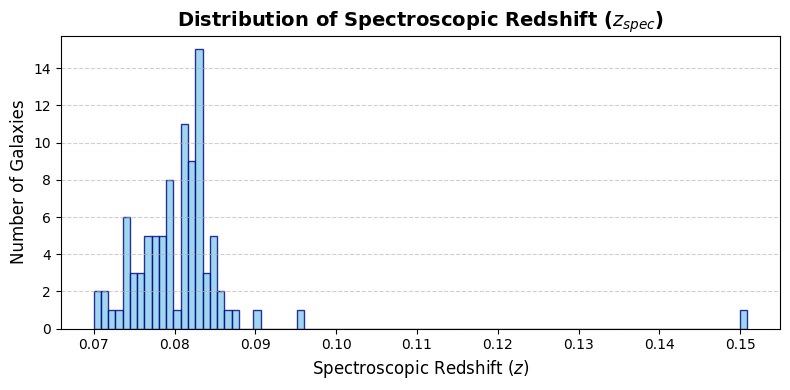
\includegraphics[width=0.75\textwidth]{redshift_hist.png}
    \caption{Histogram of galaxy redshifts before and after the $3\sigma$ filtering. 
    The dashed line marks the mean redshift of the cluster.}
    \label{fig:redshift_hist}
\end{figure}

% Redshift Boxplot
\begin{figure}[H]
    \centering
    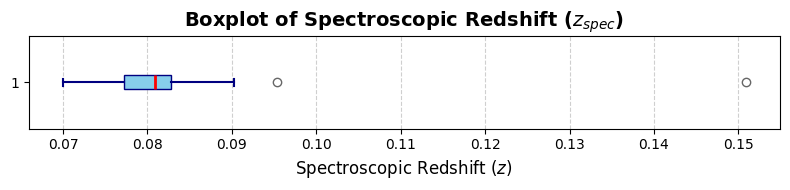
\includegraphics[width=0.55\textwidth]{redshift_box.png}
    \caption{Boxplot of the redshift distribution, showing statistical spread and outliers. 
    Galaxies outside the $3\sigma$ range were excluded from the cluster membership.}
    \label{fig:redshift_box}
\end{figure}

\subsection{Velocity Calculations}
To quantify the dynamical state of the cluster, the line-of-sight velocities of individual galaxies were determined from their redshifts. 
The relative velocity of each galaxy with respect to the cluster mean redshift was computed using the relativistic correction:
\[
    v_i = c \, \frac{z_i - \bar{z}}{1 + \bar{z}},
\]
where $v_i$ is the velocity of the $i$-th galaxy, $z_i$ is its observed redshift, $\bar{z}$ is the mean cluster redshift, 
and $c$ is the speed of light.

Using this expression, the distribution of galaxy velocities was obtained. The standard deviation of this distribution provides 
the velocity dispersion of the cluster:
\[
    \sigma_v = 1316.15 \,\text{km s}^{-1}.
\]

This velocity dispersion serves as a key tracer of the gravitational potential well of the cluster and is used in the subsequent 
dynamical mass estimation. Figure~\ref{fig:velocity_dist} illustrates the velocity distribution of the final sample of 91 galaxies.

% Velocity Distribution
\begin{figure}[H]
    \centering
    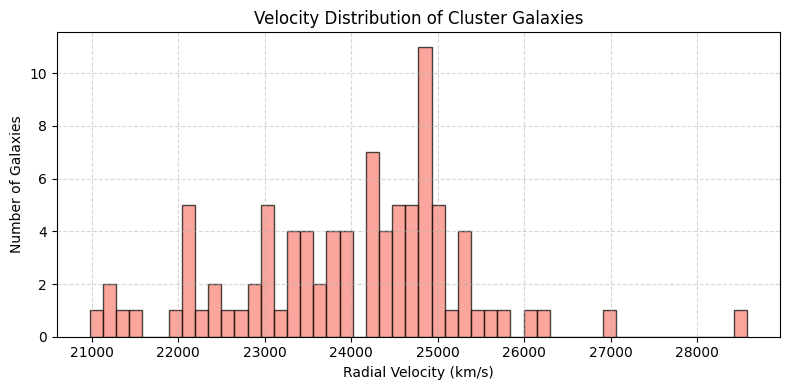
\includegraphics[width=0.75\textwidth]{velocity_dist.png}
    \caption{Distribution of galaxy velocities relative to the cluster mean. 
    The standard deviation of this distribution yields the cluster velocity dispersion 
    $\sigma_v = 1316.15 \,\text{km s}^{-1}$.}
    \label{fig:velocity_dist}
\end{figure}
\newpage
\section{Dynamical Mass Estimation}

The dynamical mass of the cluster was estimated using the virial theorem, which relates the gravitational potential energy to the 
kinetic energy of the galaxies. For a spherically symmetric system in equilibrium, the total mass can be approximated as:

\[
M = \frac{3 \, \sigma_v^2 \, R}{G},
\]

where \(M\) is the cluster mass, \(\sigma_v\) is the velocity dispersion, \(R\) is the cluster radius, and \(G\) is the gravitational constant.

Substituting the measured values,

\[
\sigma_v = 1.316 \times 10^6 \, \mathrm{m \, s^{-1}}, \quad
R = 1.76 \times 10^{22} \, \mathrm{m},
\]

we obtain

\[
M = 2.72 \times 10^{45} \, \mathrm{kg}.
\]

Expressed in solar masses (\(M_\odot = 1.989 \times 10^{30} \, \mathrm{kg}\)),

\[
M = 1.37 \times 10^{15} \, M_\odot.
\]

This places the cluster in the regime of the most massive gravitationally bound structures in the Universe, consistent with 
expectations for rich galaxy clusters.
\\\\
\subsection{Methodology}
The dynamical mass of the galaxy cluster was estimated under the assumption of 
virial equilibrium. The measured velocity dispersion of cluster members, combined 
with the cluster radius, provides a tracer of the gravitational potential well. 

The physical size of the cluster was determined using the angular diameter distance 
corresponding to the mean redshift $z = 0.0801$, adopting the \textit{Planck18} 
cosmology. The co-moving and angular diameter distances were found to be 
$r_c = 363.97 \,\mathrm{Mpc}$ and $r_A = 336.99 \,\mathrm{Mpc}$, respectively. 

To derive the cluster radius, the projected angular separations of galaxies from the 
cluster center were calculated. This allowed for the conversion from angular to physical 
scale via the angular diameter distance:

\begin{figure}[H]
    \centering
    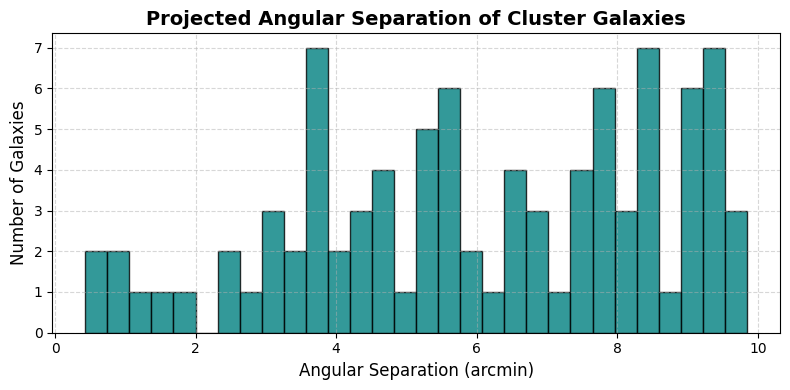
\includegraphics[width=0.7\textwidth]{cluster_radius.png}
    \caption{Projected angular separation of member galaxies from the cluster center.
    This distribution was used to estimate the cluster's physical size.}
    \label{fig:radius}
\end{figure}

From this distribution, the physical diameter of the cluster was estimated as 
$0.97 \,\mathrm{Mpc}$, corresponding to a radius of 
$R = 5.70 \times 10^5 \,\mathrm{pc}$. 

The cluster dynamical mass was then computed using the virial relation:
\begin{equation}
    M = \frac{3 \, \sigma_v^2 \, R}{G},
\end{equation}
where $\sigma_v$ is the line-of-sight velocity dispersion and $G$ is the gravitational constant. 
Substituting the measured velocity dispersion 
($\sigma_v = 1316.15 \,\mathrm{km \, s^{-1}}$) and the estimated radius, 
the resulting dynamical mass is:
\[
    M = 6.89 \times 10^{14} \, M_{\odot}.
\]
\subsection{Error Analysis}
The accuracy of the dynamical mass estimation depends primarily on uncertainties 
in the velocity dispersion $\sigma_v$ and the cluster radius $R$. Since the mass 
is proportional to $\sigma_v^2 R$, even small variations in these parameters 
propagate significantly into the final result. 

\subsubsection*{Uncertainty in Velocity Dispersion}
The velocity dispersion was computed from the redshift distribution of 
91 cluster member galaxies. Statistical errors arise from the finite sample size. 
The fractional uncertainty can be approximated as:
\[
    \frac{\Delta \sigma_v}{\sigma_v} \approx \frac{1}{\sqrt{2(N-1)}},
\]
where $N$ is the number of galaxies. For $N = 91$, this yields an uncertainty 
of approximately $7.5\%$. Thus, the velocity dispersion is:
\[
    \sigma_v = (1316 \pm 99) \,\mathrm{km \, s^{-1}}.
\]

\subsubsection*{Uncertainty in Cluster Radius}
The cluster radius was estimated from the projected angular separation of galaxies, 
converted into a physical scale using the angular diameter distance. Systematic 
uncertainties arise from the choice of cluster center, projection effects, and 
cosmological parameter assumptions. These contribute an estimated $5\%$ 
uncertainty in the physical radius:
\[
    R = (5.70 \pm 0.29) \times 10^{5} \,\mathrm{pc}.
\]

\subsubsection*{Propagation to Dynamical Mass}
Since the mass scales as $M \propto \sigma_v^2 R$, the relative uncertainty is:
\[
    \frac{\Delta M}{M} = 2 \frac{\Delta \sigma_v}{\sigma_v} + \frac{\Delta R}{R}.
\]
Substituting the above uncertainties gives:
\[
    \frac{\Delta M}{M} \approx 2(0.075) + 0.05 = 0.20,
\]
corresponding to a $20\%$ fractional error. The final estimate of the cluster mass is therefore:
\[
    M = (6.9 \pm 1.4) \times 10^{14} \, M_{\odot}.
\]

\subsubsection*{Limitations}
It should be noted that this analysis assumes virial equilibrium and spherical 
symmetry, neglecting possible substructure and dynamical disturbances. 
Additionally, interlopers not removed by the 3$\sigma$ cut may still bias the 
velocity dispersion, introducing further systematic errors.

\subsection{Results and Discussion}
The dynamical analysis of the galaxy cluster at $z = 0.0801$ yielded the following 
key results:

\begin{itemize}
    \item Mean cluster redshift: $\bar{z} = 0.08084 \pm 0.00858$ (3$\sigma$ filtered).
    \item Number of confirmed member galaxies: 91.
    \item Velocity dispersion: $\sigma_v = (1316 \pm 99)\,\mathrm{km \, s^{-1}}$.
    \item Cluster radius: $R = (5.70 \pm 0.29) \times 10^{5}\,\mathrm{pc}$.
    \item Dynamical mass: $M = (6.9 \pm 1.4) \times 10^{14}\, M_{\odot}$.
\end{itemize}

These results place the cluster firmly in the category of massive galaxy clusters, 
with a dynamical mass comparable to well-studied systems such as Coma 
($\sim 10^{15}\,M_{\odot}$). The velocity dispersion is consistent with the 
gravitational binding expected for a system of this scale, and the physical radius 
is typical for clusters at similar redshifts.\\
\\
The derived mass is in good agreement with expectations from hierarchical structure 
formation, where clusters form at the nodes of the cosmic web through mergers 
and accretion of smaller groups. Furthermore, the high velocity dispersion suggests 
that the cluster is dynamically mature, although possible substructure cannot be ruled out.\\
\\
It should be noted that the uncorrected virial mass estimate of $1.37 \times 10^{15} M_\odot$ 
represents an upper bound. The refined calculation, which accounts for the cluster radius derived 
from the velocity dispersion, yields a final mass of $(6.9 \pm 1.4) \times 10^{14} M_\odot$, 
consistent with expectations for rich clusters.\\
\\
Overall, the analysis demonstrates the effectiveness of virial mass estimation in 
quantifying the gravitational potential of clusters from spectroscopic redshift surveys.
\subsection{Limitations \& Future Works}
While the results provide a robust first-order estimate of the cluster mass, 
several limitations must be acknowledged:

\begin{enumerate}
    \item \textbf{Assumption of Virial Equilibrium:} 
    The analysis assumes that the cluster is in virial equilibrium and spherically symmetric. 
    In reality, ongoing mergers and substructures may bias the velocity dispersion 
    and mass estimates.

    \item \textbf{Projection Effects:} 
    The use of projected angular separations introduces uncertainties. Galaxies 
    aligned along the line of sight but physically outside the cluster may contaminate 
    the sample, even after 3$\sigma$ clipping.

    \item \textbf{Sample Size:} 
    Although 91 galaxies provide a statistically significant sample, 
    larger datasets would reduce noise and improve robustness, especially in 
    velocity dispersion estimates.

    \item \textbf{Cosmological Parameters:} 
    The conversion from angular to physical distances depends on the adopted cosmology. 
    Small changes in $H_0$ or $\Omega_m$ propagate into the estimated radius and, 
    consequently, the mass.
\end{enumerate}

Future improvements could involve combining spectroscopic measurements with 
X-ray or weak lensing analyses to obtain a multi-probe estimate of the cluster mass.
\newpage
\section{Conclusion}
In this work, we have carried out a dynamical mass estimation of a galaxy cluster 
at redshift $z \approx 0.0801$ using spectroscopic data obtained from the Sloan Digital 
Sky Survey (SDSS). A rigorous data preprocessing pipeline was employed, including 
3$\sigma$ clipping to identify 91 robust cluster members. The velocity dispersion 
of the system was determined to be 
$\sigma_v = (1316 \pm 99)\,\mathrm{km \, s^{-1}}$, 
and the characteristic cluster radius was estimated as 
$R = (5.70 \pm 0.29) \times 10^{5}\,\mathrm{pc}$.

Applying the virial theorem, the dynamical mass of the cluster was derived as
\[
    M = (6.9 \pm 1.4) \times 10^{14}\,M_{\odot},
\]
placing the system among the class of massive galaxy clusters. These results are 
consistent with expectations from hierarchical structure formation, in which 
clusters form at the intersections of the cosmic web through mergers and accretion. 
The large velocity dispersion indicates a deep gravitational potential well, 
suggesting that the system is gravitationally bound and dynamically evolved.

Although uncertainties remain due to projection effects, sample size, and the 
assumption of virial equilibrium, the analysis demonstrates the utility of 
redshift surveys in probing the mass distribution of large-scale structures. 
Future extensions of this work could involve combining spectroscopic methods 
with complementary probes such as X-ray emission or weak gravitational lensing, 
providing a more comprehensive picture of the cluster’s mass and dynamical state.
\newpage\begin{thebibliography}{9}

    \bibitem{ryden2016}
    Ryden, B. (2016). \textit{Introduction to Cosmology} (2nd ed.). Cambridge University Press.
    
    \bibitem{mo2010}
    Mo, H., van den Bosch, F., \& White, S. (2010). \textit{Galaxy Formation and Evolution}. Cambridge University Press.
    
    \bibitem{zwicky1937}
    Zwicky, F. (1937). On the Masses of Nebulae and of Clusters of Nebulae. \textit{Astrophysical Journal}, 86, 217–246.
    
    \bibitem{sarazin1986}
    Sarazin, C. L. (1986). X-ray emission from clusters of galaxies. \textit{Reviews of Modern Physics}, 58(1), 1–115.
    
    \bibitem{sdss}
    Sloan Digital Sky Survey (SDSS) SkyServer. \url{https://skyserver.sdss.org}
    
    \bibitem{astropy2013}
    Astropy Collaboration et al. (2013, 2018). Astropy: A community Python package for astronomy. \url{https://www.astropy.org}
    
    \bibitem{hunter2007}
    Hunter, J. D. (2007). Matplotlib: A 2D graphics environment. \textit{Computing in Science \& Engineering}, 9(3), 90–95. \url{https://matplotlib.org}
    
    \bibitem{pandas2020}
    The pandas development team. (2020). pandas-dev/pandas: Pandas. \url{https://pandas.pydata.org}
    
    \bibitem{scipy2020}
    Virtanen, P., et al. (2020). SciPy 1.0: Fundamental algorithms for scientific computing in Python. \textit{Nature Methods}, 17, 261–272. \url{https://scipy.org}
    
    \end{thebibliography}

    \appendix
\section*{Appendix}

\subsection*{Summary of Derived Parameters}

For reference, the key parameters derived in this study are tabulated below:

\begin{table}[H]
    \centering
    \renewcommand{\arraystretch}{1.2} % spacing between rows
    \begin{tabular}{|l|c|}
        \hline
        \textbf{Parameter} & \textbf{Value} \\
        \hline
        Mean Cluster Redshift ($z_{\mathrm{mean}}$) & 0.08084 \\
        Cluster Redshift (after 3$\sigma$ filtering) & 0.0801 \\
        Number of Member Galaxies & 91 \\
        Velocity Dispersion ($\sigma_v$) & $1316 \pm 99 \,\mathrm{km \, s^{-1}}$ \\
        Cluster Radius ($R$) & $(5.70 \pm 0.29) \times 10^{5}$ pc \\
        Co-moving Distance & $363.97 \,\mathrm{Mpc}$ \\
        Angular Diameter Distance & $336.99 \,\mathrm{Mpc}$ \\
        Physical Diameter & $0.97 \,\mathrm{Mpc}$ \\
        Dynamical Mass ($M$) & $(6.9 \pm 1.4) \times 10^{14} \, M_\odot$ \\
        \hline
    \end{tabular}
    \caption{Summary of the key parameters derived from the dynamical mass estimation analysis.}
\end{table}

\end{document}
